\newpage
\section{Significance and Limit calculation}
\label{sec:limits}
This 
section will describe the test statistic to evaluate the conformity with 
background of the measured alerts.
% if the measured alerts are 
% background conform or can be attributed to a signal source.
The test statistic is based on multiplying the p-values of different 
components which can be separated into two categories: the pure number of 
alerts and the probability that doublets stem from background.

The Optical Follow-Up was designed with the expectation that most of the alerts 
will be triggered due to background events of atmospheric neutrinos. An excess 
of detected multiplets in comparison to the expected background 
average can indicate a possible signal contribution. 

Given the average 
background expectation (Section ???) $\mu_{k,b}$ for multiplets with 
multiplicity $k$, the probability to see $N_k$ or more alerts during one 
season is
\begin{equation}
 P(N_k, \mu_k) = \sum P_\text{Poisson} = \sum_{i=N_k}^\infty 
\frac{\mu_k^i}{i!}\exp^{-\mu_k}.
\end{equation}
The sum is aborted when a precision of $10^{-6}$ is reached.
The probabilities for the different multiplicities $k$ and seasons $i$ are then 
multiplied to form the test statistic $\lambda_{na}$ to evaluate the number of 
alerts
\begin{equation}
\label{eq:test_statistic}
 \lambda_{na} \left(N_k^i, \mu_{k,b}^i \right) = \prod_{k=2}^\infty \prod_i 
P(N_k^i, 
\mu_{k,b}^i).
\end{equation}

The second component is only valid for doublets as higher multiplicities are 
automatically considered true alerts. The OFU system generates up to about 50 
doublets per year of which only seven can be sent to Swift. The down selection 
is based on the OFU test statistic (Section ???) separating the more signal 
like and the more background like doublets. For each doublet an OFU test 
statistic value is drawn and compared to the background distribution to 
calculate the p-value $p_{j, i}^{ofu}$. The p-values of all doublets can not 
simply be multiplied as the number of doublets would influence the significance 
of the test statistic. E.g. three background doublets would form a smaller 
overall p-value $O(10^{-3})$ than one signal doublet $O(10^{-1})$. A combination 
of all $p_{j,i}^{ofu}$ was chosen to keep the total contribution in the same 
order of magnitude independent of the number of doublets.
%order as the contributions of the amount of multiplets per multiplicities and 
%season $P(N_k^i, \mu_{k,b}^i)$ by multiplying i
All $p_{j,i}^{ofu}$ are multiplied and 
the ${N_2^i}^{th}$ square root is taken of the product with $N_2^i$ being the 
number of considered 
doublets of season $i$
\begin{equation}
\label{eq:lambda_ofu}
 \lambda_\text{ofu} = \prod_i \sqrt[N_2^i]{\prod_{j=1}^{N_2^i} p_{j,i}^{ofu}}
\end{equation}
Calculating $p_{j,i}^{ofu}$ is based on several steps. The OFU test statistic 
distribution differs slightly for different zenith regions. To evaluate the 
correct test 
statistic a zenith value is drawn for each doublet according to the squared 
singlet rate (Figure \ref{fig:cos_zen_prob_dens_bg_IC86_BDT}, 
\ref{fig:cos_zen_prob_dens_sg2p3_IC86_BDT}). 

\begin{figure}[h]
\centering
 \captionsetup{width=.85\textwidth}
%  \captionsetup{margin=0pt}
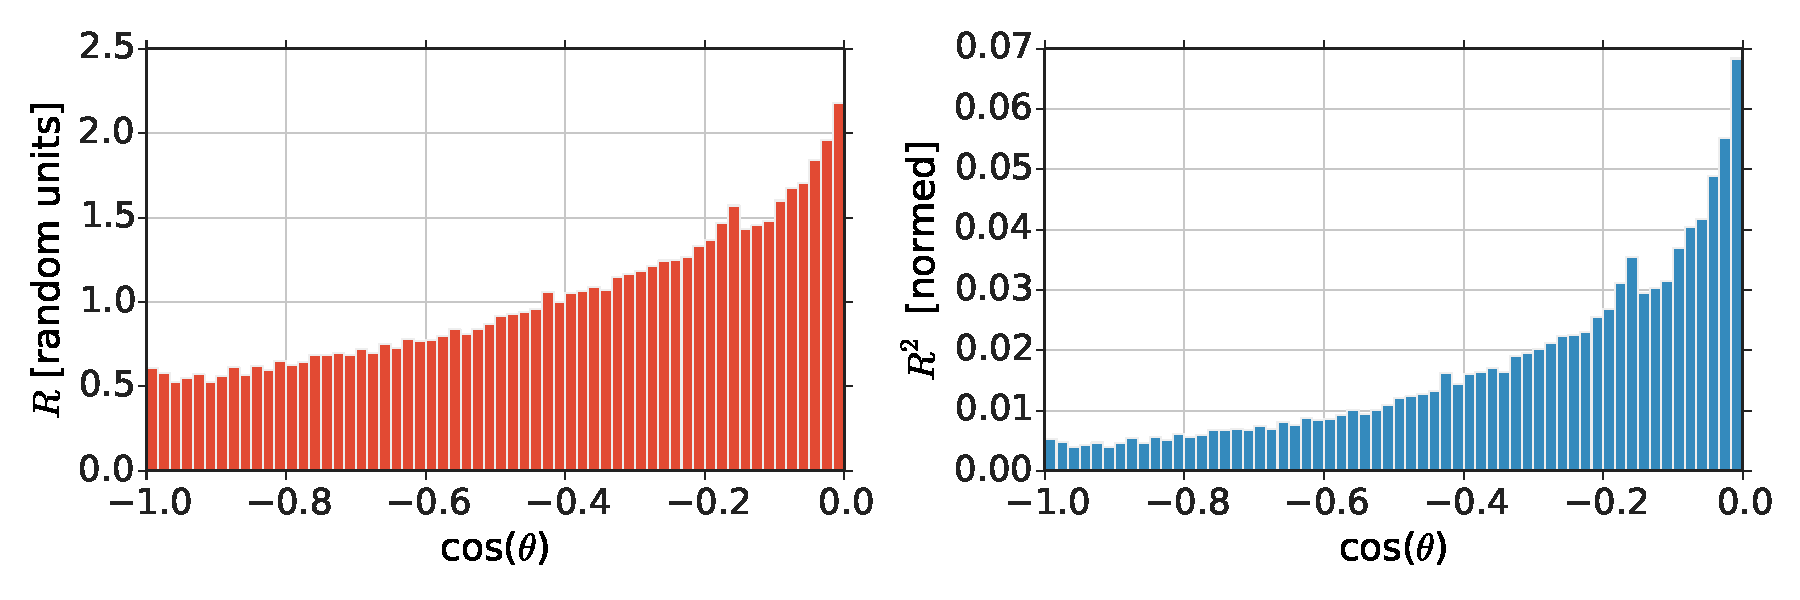
\includegraphics[width=0.85\textwidth]{%
fig/cos_zen_prob_dens_bg_IC86_BDT.pdf}
 \caption{The plots show the cosinus zenith distribution for background of the 
IC86-BDT season. The left plot depicts the singlet rate in random units and the 
right plot is the probability density function of the doublet distribution 
(singletrate squared)}
\label{fig:cos_zen_prob_dens_bg_IC86_BDT}
\end{figure}

\begin{figure}[h]
\centering
 \captionsetup{width=.85\textwidth}
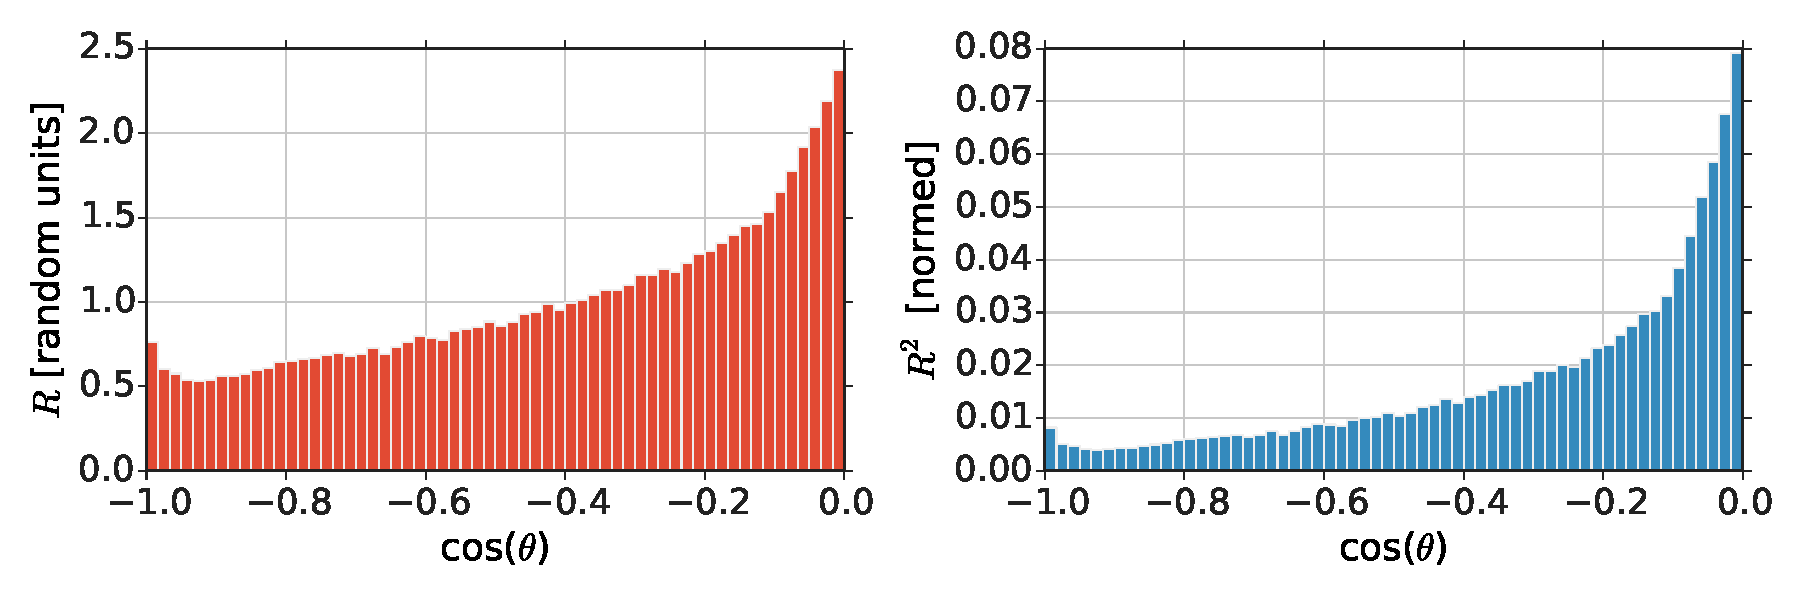
\includegraphics[width=0.85\textwidth]{%
fig/cos_zen_prob_dens_sg2p3_IC86_BDT.pdf}
\caption{The plots show the cosinus zenith distribution for signal with a 
spectral index of $\gamma=2.3$ of the 
IC86-BDT season. The left plot depicts the singlet rate in random units and the 
right plot is the probability density function of the doublet distribution 
(singletrate squared)}
\label{fig:cos_zen_prob_dens_sg2p3_IC86_BDT}
\end{figure}
The northern sky was divided 
into twenty even regions in $\cos(\theta)$ and the probability density 
functions of the OFU test statistic were created for background and signal of 
all considered spectra for all seasons in each region. An example is shown 
in Figure \ref{fig:ofu_teststat_zone00_IC86_BDT_bg_g2p3} for the first zone 
from the pole for the IC86-BDT season. Using the zenith value the correct OFU 
test statistic probability density function is chosen to draw a test statistic 
value. As the probability to have a Swift doublet is already included in 
calculating the expected number of doublets $\mu_{2}^i$, the test statistic 
value must be smaller than the Swift cut of the season. The chosen value is 
then compared to the cumulative background distribution (Figure 
\ref{fig:ofu_teststat_zone00_IC86_BDT_bg_cum}) and the p-value is extracted.

\begin{figure}[h]
\centering
 \captionsetup{width=.4\textwidth}
%  \captionsetup{margin=0pt}
 \subfloat[The probability density functions of the OFU test statistic 
(background and signal with a spectral index of $\gamma=2.3$) for the first 
region starting from the pole for the IC86-BDT season. 
\label{fig:ofu_teststat_zone00_IC86_BDT_bg_g2p3}]{%
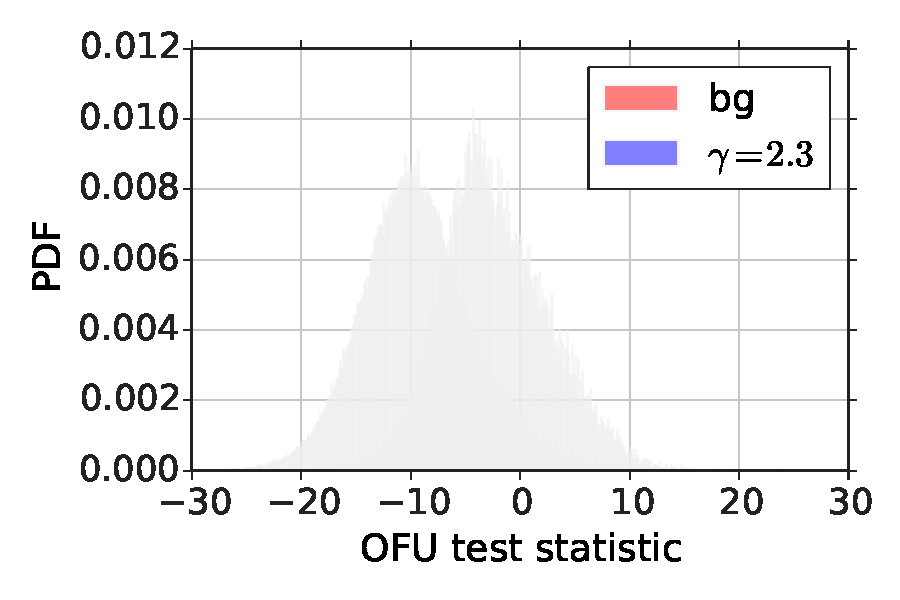
\includegraphics[width=0.45\textwidth]{%
fig/ofu_teststat_zone00_IC86_BDT_bg_g2p3.pdf}}
\subfloat[The cumulative 
distribution of the background 
OFU test statistic for the 
IC86-BDT season.\label{fig:ofu_teststat_zone00_IC86_BDT_bg_cum}]{%
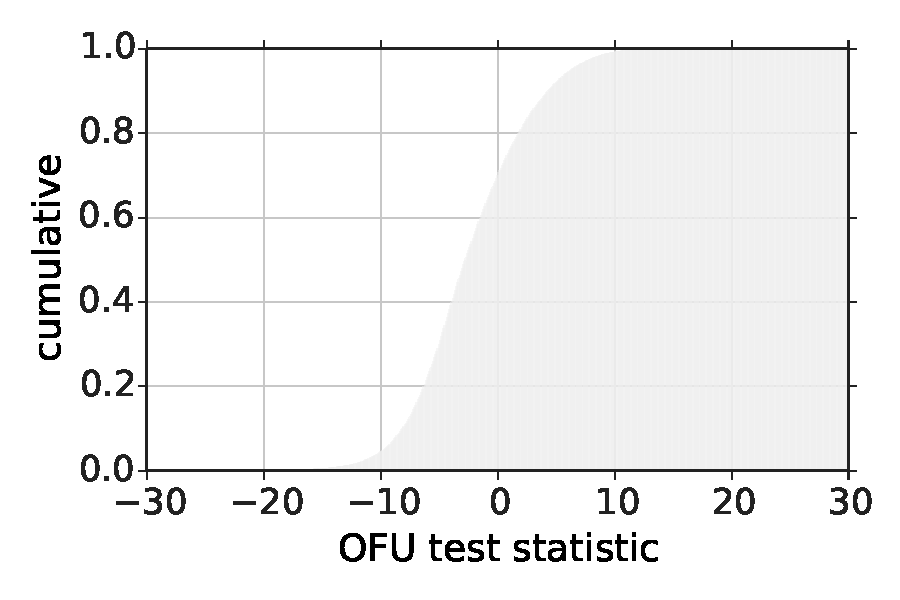
\includegraphics[width=0.45\textwidth]{%
fig/ofu_teststat_zone00_IC86_BDT_bg_cum.pdf}}
\end{figure}

The complete test statistic is the combination of both components
\begin{equation}
\label{eq:lam_total}
 \lambda = \lambda_{na} \cdot \lambda_\text{ofu}
\end{equation}


The final significance and limit calculation is based on running pseudo 
experiments. To evaluate the 
agreement of the measured alerts with a pure background hypothesis, the average 
background expectation $\mu_{k, b}^i$
per season $i$ and multiplicity $k$  is used to draw a number of 
detected multiplets $N_k^i$ according to a Poisson distribution. 
For all $N_2^i$ doublets, $p_{j,i}^{ofu}$ is calculated. 
In total, 
$10^6$ experiments are performed per season and the resulting 
 test statistic values are compared to the measured result ($\lambda_m$). The 
p-value is the fraction of experiments with worse agreement to the background 
hypothesis ($\lambda < \lambda_m$).


Similarly, a signal hypothesis can be tested. The GRB Toy Monte Carlo is used 
to estimate the average number of expected multiplets $\mu_{k,s, \gamma}^i$ for 
a 
specific model and $N_{k,s, \gamma}^i$ values are again generated according to 
the 
Poisson  distribution. The number of alerts $N_{k,s+b}^i$ is the
combination of background and signal alerts
\begin{equation}
 N_{k,s+b}^i = N_{k,s}^i + N_{k,b}^i.
\end{equation}
The influence of the OFU test statistic (Eq. \ref{eq:lambda_ofu}) is 
\begin{equation}
 \lambda_\text{ofu} = \prod_i \sqrt[N_{2,s+b}^i]{\prod_{j=1}^{N_{2,b}^i} 
p_{j,i,b}^{ofu} \cdot \prod_{j=1}^{N_{2,s}^i}
p_{j,i,s}^{ofu}}
\end{equation}

Again, $10^6$ experiments are performed per season and GRB 
model and the test statistic (Eq. \ref{eq:lam_total})
% $\lambda\left(N_{k,s+b}^i, \mu_{k,b}^i \right)$
evaluated. A model can be ruled 
out at 90\% confidence level if 90\% of the experiments show a worse agreement 
with the background only hypothesis than the actual experimental results.
An example is shown in Figures \ref{fig:test_statistic} and 
\ref{fig:test_statistic_cumulative}.
\begin{figure}[h]
\centering
 \captionsetup{width=.9\textwidth}
%  \captionsetup{margin=0pt}
\subfloat[Differential distribution\label{fig:test_statistic}]{%
 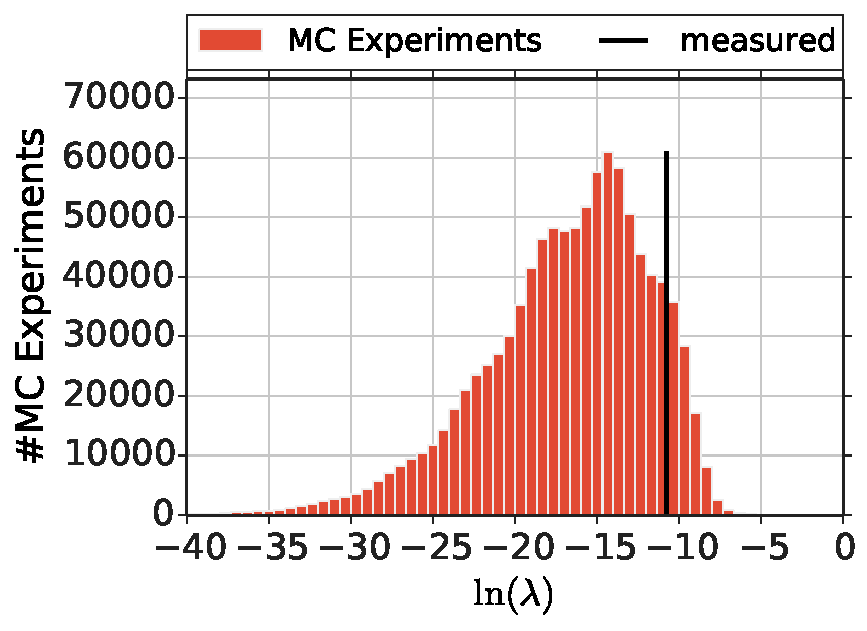
\includegraphics[width=0.45\textwidth]{fig/test_statistic.pdf}}
 \subfloat[cumulative distribution\label{fig:test_statistic_cumulative}]{%
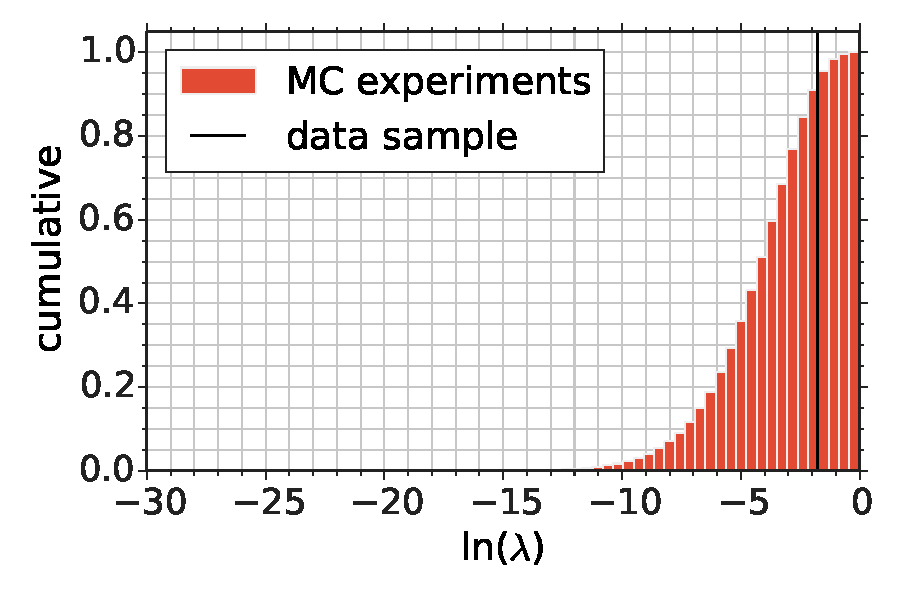
\includegraphics[width=0.45\textwidth]{fig/test_statistic_cumulative.pdf}}
\caption{$10^6$ experiments were thrown and the 
test statistic $\lambda$ was calculated according 
to equation \ref{eq:test_statistic}. In read is the differential
distribution of the Monte Carlo experiments while 
the black line represents the detected value. About 90\% of the experiments 
have a worse agreement with the background only hypothesis.}
\end{figure}

% % in thesis write abortion of quadruplets in bg//????
% 
% % explain: more multiplets than expected. might be due to signal. test hypothesis 
% % that it is pure background. -> test how many experiments are less background 
% % like than measured. -> pvalue
% % 
% % the other idea: we have a model giving us a signal leading to a certain number 
% % of multiplets. if high enough, than having measured to few -> model can be 
% % excluded. for that u_k stays for background only in test statistic but is 
% % tested with N_k = N_k,s + N_k,b. hence. the signal plus bg is tested against 
% % background case. if in 90 \% of the cases the lambda is smaller means that 
% % measurement agrees better with bg than 90 \% of the experiments. only 10 \% 
% % better with bg. model can be ruled out. 
% % 
% % problem: I think that current setup uses signal + bg in lambda. Is that true. 
% % How do I then get the same exclusion regions as nora? in that case shouldn't be 
% % 0.1 be the 90\% exclusion?
% 
% 
% In this section the test test statistic and the Toy Monte Carlo are explained 
% that are used to test the hypothesis that the experimental data is pure 
% background and to limit the possible contribution of a neutrino signal due to 
% a 
% transient source.
% 
% The Toy Monte Carlo runs $10^6$ experiments drawing a number of alerts $N_k$ 
% according to a Poisson distribution with a given mean expectation of $\mu_k$.
% % Given an average expectation value $\mu_k$ of alerts with a multiplicity $k$, 
% % a 
% % number of alerts $N_k$ are drawn according to the Poisson distribution $10^6$ 
% % times for each season.
% For each experiment 
% \begin{equation}
%  P(N_k, \mu_k) = \sum P_\text{Poisson} = \sum_{i=N_k}^\infty 
% \frac{\mu_k^i}{i!}\exp^{-\mu_k}
% \end{equation}
% describes the probability to detect $N_k$ or more alerts. The sum is aborted 
% when a precision of $10^{-6}$ is reached. All experiments are combined to a 
% distribution of the test statistic
% \begin{equation}
%  \lambda_\nu = \prod_{k=2}^\infty \prod_i P(N_k^i, \mu_k^i)
% \end{equation}
% in which the probabilities of each contributing seasons are multiplied per 
% multiplicity and then similarly combined with the probabilities of the 
% different types of multiplets.
% 
% In the previous section the methods to calculate an average background 
% $\mu_k^{BG}$ and a signal expectation $\mu_k^{S}$ for alerts with the 
% multiplicity $k$ has been described. 
% To limit a possible signal flux, the average expectation value is set to a 
% combination of background and signal expectation
% \begin{equation}
%  \mu_k = \mu_k^S + \mu_k^{BG}
% \end{equation}
% and the test statistic is calculated $10^6$ times as explained above and 
% compared to the value for the measured multiplets rate $\lambda_m$. A model 
% can be ruled out with the probability of the fraction $x$ of experiments 
% which show a worse agreement with the hypothesis, e.g. with a smaller test 
% statistic value than the measured data.
% An example is shown in Figures \ref{fig:test_statistic} and 
% \ref{fig:test_statistic_cumulative} in which the signal hypothesis is ruled out 
% at a 90\% confidence level.
% \begin{figure}[h]
% \centering
%  \captionsetup{width=.4\textwidth}
% %  \captionsetup{margin=0pt}
% \subfloat[\label{fig:test_statistic}]{%
%  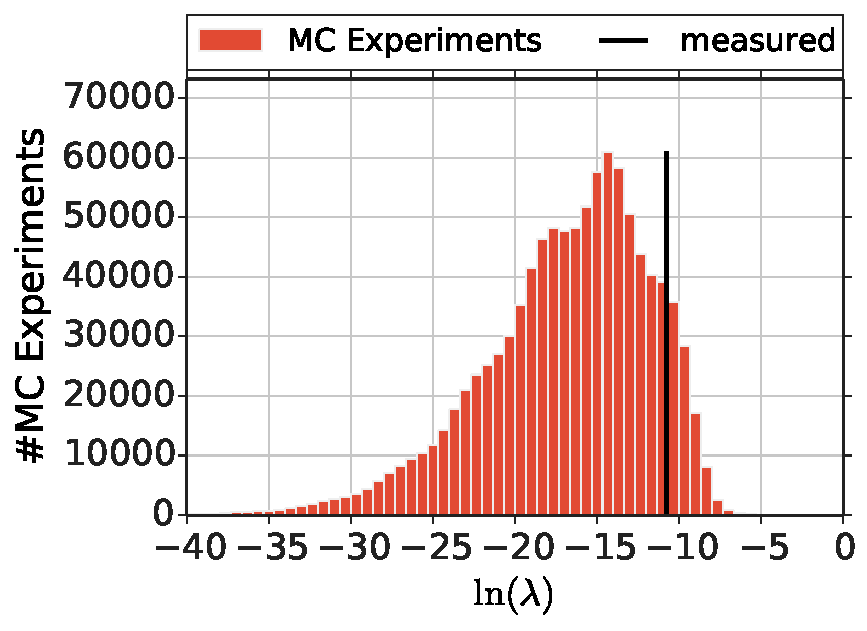
\includegraphics[width=0.45\textwidth]{fig/test_statistic.pdf}}
%  \subfloat[ 
% \label{fig:test_statistic_cumulative}]{%
% 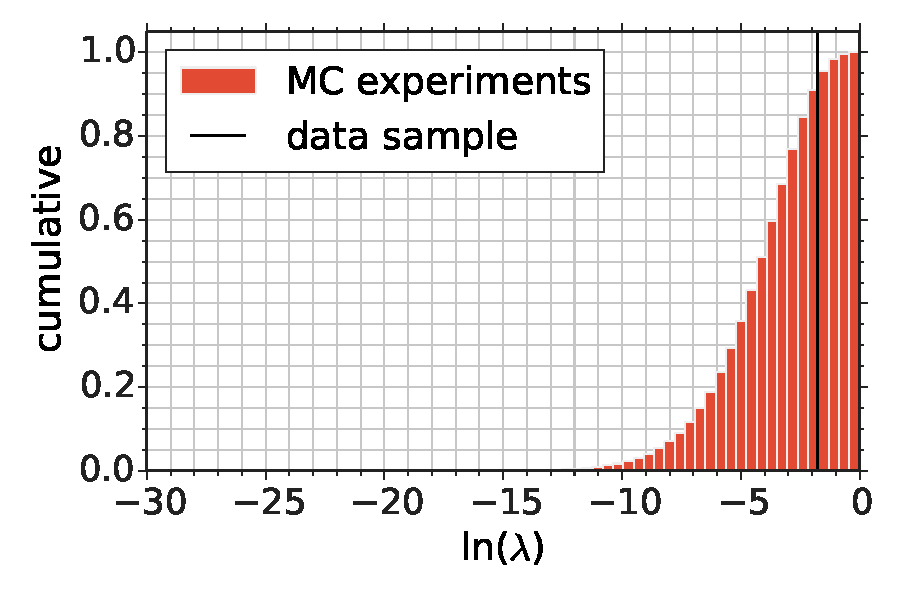
\includegraphics[width=0.45\textwidth]{fig/test_statistic_cumulative.pdf}}
% \end{figure}
% 
% Similarly, the sensitivity to the pure background hypothesis can be tested by 
% setting 
% \begin{equation}
%  \mu_k = \mu_k^{BG}
% \end{equation}
% and rerunning the Toy Monte Carlo. A possible signal contribution becomes 
% likely if few experiments have a worse agreement with the background assumption 
% meaning a value less than the measured 
% 
%  significance  The p-value is the 
% fraction of experiments that agree worse with this hypothesis than the data 
% taken, i.e. the experiments with a value smaller than $\lambda_m$.